% !TeX TXS-program:compile = txs:///pdflatex/[--shell-escape] %

\documentclass[a4paper,oneside,11pt]{scrreprt}
\usepackage{listings} % Essential for typesetting code snippets
% This document class 'scrreprt' is suitable for reports and theses, providing 'chapter' as the highest sectioning level.
% For shorter works, 'scrartcl' could be used, where 'section' is the highest level (no 'chapter').
% \documentclass[a4paper,bibtotoc,oneside]{scrbook} % Another option for books/theses with bibliography in ToC

\usepackage[utf8]{inputenc} % For proper handling of UTF-8 characters
\usepackage{amsmath} % Provides environments for equations (e.g., align, gather) and math commands
\usepackage{amsfonts} % Provides additional math fonts (e.g., blackboard bold)
\usepackage{amssymb} % Provides additional math symbols
\usepackage{graphicx} % For including images (e.g., diagrams if you add them later)
\usepackage{amsthm} % Provides environments for theorems, definitions, etc. (optional, but good practice)
\usepackage{physics} % A useful package for common physics notations, like \qty for quantity and unit
\usepackage{siunitx} % For proper typesetting of units (e.g., \SI{15}{\degree})
\usepackage{geometry} % For easily setting page margins and dimensions
\usepackage{xcolor} % For custom colors, often used with listings for syntax highlighting

\usepackage{booktabs}
\usepackage{multirow}

% --- Custom Settings for Code Listings ---
% This block defines how your code snippets will look.
\lstset{
    basicstyle=\ttfamily\small,     % Font style for the code (monospace, small size)
    columns=fullflexible,           % Allows flexible column width, good for long lines
    breaklines=true,                % Enables automatic line breaking for long lines
    tabsize=4,                      % Sets the number of spaces for a tab character
    showstringspaces=false,         % Don't show special characters for spaces in strings
    commentstyle=\color{gray},      % Color for comments in the code
    keywordstyle=\color{blue},      % Color for programming language keywords
    stringstyle=\color{purple},     % Color for string literals
    numbers=left,                   % Places line numbers on the left side of the code block
    numberstyle=\tiny\color{gray},  % Style for the line numbers (tiny, gray)
    frame=single,                   % Draws a single frame around the code block
    frameround=!!!!,                % Makes the corners of the frame rounded
    rulesepcolor=\color{gray},      % Color of the separator line between the frame and the code
    backgroundcolor=\color{white},  % Background color of the code block
    captionpos=b,                   % Positions the caption below the code block (b for bottom)
    breakatwhitespace=true,         % Allows line breaks at whitespace
    % Specific to C++ language highlighting
    language=C++,
    morekeywords={JointAngles, constrain_value, static_cast}, % Custom keywords to highlight
    literate={*}{{$\cdot$}}1        % Replaces '*' with a multiplication dot symbol
}
% --- End of Custom Settings for Code Listings ---

% --- Language and Encoding Settings ---
\usepackage[utf8]{inputenc} % Ensures proper handling of UTF-8 characters
\usepackage{ifthen} % Provides conditional commands
\newboolean{english}
\setboolean{english}{true} % Set to 'true' for English version, 'false' for German

% --- Core LaTeX Packages ---
\usepackage{amsmath} % Provides advanced mathematical environments and commands
\usepackage{amsfonts} % Provides additional mathematical fonts (e.g., blackboard bold)
\usepackage{amssymb} % Provides additional mathematical symbols
\usepackage{graphicx} % Enables inclusion of images
\usepackage{booktabs} % Enhances the appearance of tables with professional rules (toprule, midrule, bottomrule)
\usepackage{caption}  % Provides enhanced caption customization for figures and tables
\usepackage{multirow} % Add this line
% --- TikZ for Diagrams ---
\usepackage{tikz} % Main package for creating vector graphics
\usetikzlibrary{shapes,arrows,positioning,calc}

% Define TikZ styles for consistency across all diagrams in the document

% Define TikZ styles for consistency across all diagrams in the document
\tikzset{
    block/.style={
        rectangle,
        draw,
        fill=blue!10,
        text width=5em,
        text centered,
        rounded corners,
        minimum height=2.5em,
        font=\small % Added from the second block, ensuring it's applied
    },
    sum/.style={
        draw,
        circle,
        node contents={+},
        inner sep=1pt, % Adjust inner padding
        minimum size=1.5em % Adjust size of the circle
    },
    input/.style={coordinate},
    output/.style={coordinate},
    arrow/.style={
        -latex,
        thick
    },
    disturbance/.style={
        -latex,
        dashed, % Use dashed line for disturbance path
        thick,
        red!70!black % Optional: color for disturbance
    },
    line/.style={ % This style was only in the second block, now correctly included
        draw,
        -latex' % A simpler arrow for direct connections
    }
}

% --- Thesis-Specific Definitions (Metadata) ---
\def\title{Implementing Adaptive Control in ROS 2 for a Laparoscopic Surgical Robotic Test Platform}
%\def\title{Title of the Thesis} % Uncomment and modify for a different title
\def\study{Mechatronics and Smart Technologies - Mechanical Engineering}
%\def\study{Mechatronik - Elektrotechnik} % Uncomment and modify for a different study program
\def\thesis{Master Thesis}
%\def\thesis{Bachelorarbeit 2} % Uncomment and modify for a different thesis type
\def\degree{"Master of Science in Engineering"} % Degree awarded
\def\student{Liam Nolan} % Student's name
\def\matnr{51843934} % Student's matriculation number
\def\address{6020, Innsbruck, Amraser Str. 90} % Student's address
\def\reviewerone{FH-Prof. Yeongmi Kim, PhD} % First reviewer's name and title
%\def\reviewertwo{Dr. Markus Mustermann} % Uncomment and modify for a second reviewer

% --- Inputting External Definitions ---
% Note: All TikZ definitions are now directly in this file.
% If 'etc/definitions.tex' contains other non-TikZ specific definitions,
% keep the following line. Otherwise, it can be removed if empty.
% deutsche Anpassungen
%\usepackage[ansinew]{inputenc}
\usepackage[T1]{fontenc}
\usepackage[ngerman,english]{babel}
%\usepackage{babelbib}

% mathematische Symbole
\usepackage{amsmath,amssymb,amsfonts,amstext}

% Listings
\usepackage{listings}
\lstset{numbers=left,numberstyle=\tiny,stepnumber=5,numbersep=5pt}

% erweiterte Zeichenbefehle
\usepackage{pst-all}

% Kopfzeilen frei gestaltbar
\usepackage{fancyhdr}
 

% Farben im Dokument m"oglich
\usepackage{color}

% Schriftart Helvetica
\usepackage{helvet}
\renewcommand{\familydefault}{phv}

% anderdhalbfacher Zeilenabstand
\usepackage{setspace}
\onehalfspacing

% Graphiken einbinden: hier f"ur pdflatex
\usepackage{graphicx}
\usepackage{import}
\usepackage{pdfpages}

% verbesserte Floating Plazierung
\usepackage{float}

% "Uberpr"ufung des Layouts
\usepackage{layout}
\usepackage{array}  % For better table formatting

% erweiterte Einstellungen der Bildunterschriften -> 8 Pt
\usepackage{caption}
\captionsetup{font=small,belowskip=12pt,aboveskip=4pt}
\usepackage{subcaption}

% f"ur floatbarrier
\usepackage{placeins}

\usepackage{ifthen}

% H"ohe und Breite des Textk"orpers etwas gr"osser definieren

% Quellcode
\sisetup{input-digits = 0123456789\pi}%

% Referenzierung
\usepackage{hyperref}

% kreise um zahlen/Buchstaben
\newcommand{\kreis}[1]{\unitlength1ex\begin{picture}(2.5,2.5)%
\put(0.75,0.75){\circle{2.5}}\put(0.75,0.75){\makebox(0,0){#1}}\end{picture}}

% f"ur inline figures
\usepackage{scalerel}

% Einr"uckung von und Abstand zwischen Abs"atzen
\setlength{\parindent}{0em}
\setlength{\parskip}{1.5ex plus0.5ex minus0.5ex}

% weniger Warnungen wegen "uberf"ullter Boxen
\tolerance = 9999
\sloppy

% Anpassung einiger "Uberschriften 
\renewcommand\figurename{Figure}
\renewcommand\tablename{Table}
%\newcommand{\unit}{\mathrm}

% Counter f"ur die Nummerierung
\newcounter{romancount}

% Boolsche Variable f"ur Bachelor-/Masterarbeit oder Bericht
\newboolean{thesis}

% custom command for parameters
\newcommand{\param}[1]{\textit{#1}}
 % This line loads any other custom definitions (non-TikZ)

\begin{document}

\pagestyle{fancy}
\lfoot[\fancyplain{}{}]{\fancyplain{}{}}
\cfoot[\fancyplain{}{\footnotesize\thepage}]{\fancyplain{}{\footnotesize\thepage}}
\lhead[\fancyplain{}{\footnotesize
ouppercase\leftmark}]{\fancyplain{}{}}
\chead{}
\rhead[\fancyplain{}{}]{\fancyplain{}{\footnotesize
ouppercase
	ormalfont\leftmark}}

% --- Language Selection and Listing Counter ---
\ifthenelse{\boolean{english}}{\selectlanguage{english}}{\selectlanguage{ngerman}}
\counterwithin{lstlisting}{chapter} % Resets listing counter at each new chapter

%\layout % Uncomment to display the document layout (for debugging margins etc.)

% --- Page Style Setup ---
% Initiates header and footer styles for preliminary pages (Roman numbering)
\pagestyle{plain}

% --- Front Matter (Roman Numerals) ---
\pagenumbering{Roman} % Sets page numbering to Roman numerals for front matter
\input{etc/title_page.tex} % Title page content
\input{etc/liu.tex} % Likely a declaration page
\section*{\centering \ifthenelse{\boolean{english}}{Acknowledgement}{Danksagung}}
I want to thank....







\newpage
 % Acknowledgements/Thanks page
%\selectlanguage{ngerman}
%\section*{\centering Kurzfassung}
%Text Text Text Text Text Text Text Text Text Text Text Text Text Text Text Text Text Text Text Text Text Text Text Text ...

% Bitte 3-5 deutsche Schlagw"orter eingeben, die die Arbeit charakterisieren:
%\paragraph*{Schlagw"orter:} Schlagwort 1, Schlagwort 2, Schlagwort 3, Schlagwort 4, Schlagwort 5
%\newpage

\selectlanguage{english}
\section*{\centering Abstract}
The advancement of laparoscopic surgical robotics has contributed significant progress to the field of minimally invasive surgery; however, their high cost limits widespread adoption in research and training efforts. This system utilizes low-cost, off-the-shelf hardware to produce an accessible development platform for research purposes. It leverages ROS 2's distributed framework to improve real-time system performance and enable future software architecture scalability. Advanced system identification methods were employed to characterize the system, and an adaptive control strategy was implemented to compensate for varying system dynamics throughout the range of motion. Experimental validation demonstrates that the ROS 2-based architecture, in combination with the advanced system identification and control methods, provides significant performance improvements over the previous implementation. The results confirm the feasibility of a cost-effective surgical robotic system with advanced, adaptable control strategies, contributing to the advancement and accessibility of the next generation of robotic-assisted surgical systems.

\paragraph*{Keywords:} Advanced control engineering, LQR controller

\newpage
 % Abstract content

% --- Table of Contents ---
\ifthenelse{\boolean{english}}{\selectlanguage{english}}{\selectlanguage{ngerman}} % Re-select language for ToC
\tableofcontents % Generates the table of contents
\newpage % Starts a new page after the table of contents



% --- Main Body (Arabic Numerals) ---
\setcounter{romancount}{\value{page}} % Stores the last Roman page number
\setcounter{page}{1} % Resets page counter to 1
\pagenumbering{arabic} % Sets page numbering to Arabic numerals for main content

% Initiates header and footer styles for main content pages



%\selectlanguage{ngerman} % Uncomment if specific chapters need to be in German

% --- Chapter Files ---
\chapter{Introduction}


\section{Background and Context}
\label{section:background}

Laparoscopic surgery offers a minimally invasive surgical option that significantly reduces postoperative pain and recovery time for patients. However, the complex dexterity demands of this surgical technique have created a need for robotic assistance. Systems such as Intuitive Surgical’s da Vinci have been performing operations since 1999. While highly effective, these systems are prohibitively expensive and technically complex, and as a result, remain largely inaccessible to many researchers, surgeons, and clinicians. These barriers make it difficult to advance developments in the field of robotic-assisted surgery. In an effort to reduce these obstacles, researchers at MCI have previously developed a low-cost, desktop-operated surgical robotic system.

\section{Problem Statement}
\label{section:problem_statement}

While this system was effective in providing a low-cost alternative to existing solutions, its dynamic performance and software architecture left room for improvement. The software architecture was implemented using a C-based Arduino framework, which lacked many features necessary for supporting further technical advancements. Additionally, the system was controlled using a tuned PID controller which, while providing basic control over the system, left significant performance gains unrealized. The system was also highly nonlinear in nature, and as the control target deviated from the linearization point, its performance degraded considerably, resulting in inadequate control behavior.

\section{Research Aim and Objectives}
\label{section:objectives}

The goal of the research conducted in this thesis was twofold. First, to implement a ROS 2 framework for the existing system. ROS 2 is the current industry standard open-source distributed robotics middleware framework, making it well suited for the dynamic, precision-focused requirements of surgical robotic systems. Its modular nature allows for the development of multiple complex subsystems in parallel, and its framework can be easily adapted to accommodate future additions or improvements to the platform. Additionally, ROS 2 offers many essential tools for complex robotic systems, such as system visualization, collision detection, and frame transformation frameworks. Porting the existing system to this ROS 2-based framework would allow access to these benefits and facilitate further development of the system in the future.

Secondly, due to the lack of dynamic performance and control in the current system, this research aimed to develop a more robust characterization and control strategy to address its nonlinear nature. The improved characterization strategy involves comparing the results of step response experiments to closed-loop excitation data to better model the system. More advanced control strategies, such as Linear Quadratic Regulator (LQR) and Linear Quadratic Integral (LQI) controllers with feedforward control, could then be applied to this system model. Additionally, gain scheduling techniques would be utilized to adapt the controller to the system’s highly nonlinear behavior.


\section{Scope and Limitations}
\label{section:scope_limitations}

This thesis focuses on the implementation of an adaptive control framework within a ROS 2-based architecture for a laparoscopic surgical robotic test platform. The scope of the research includes the migration of the existing robotic system from a C-based Arduino framework to ROS 2, the development of advanced control strategies to address system nonlinearities, and the experimental validation of the proposed control methods using a laboratory-scale test platform.

Clinical application and in vivo testing are beyond the scope of this work; thus, the system is evaluated exclusively in controlled lab environments. The research prioritizes software architecture and control performance over hardware design improvements. Furthermore, the adaptive control methods are tested on predefined motion trajectories and system responses, which may not cover the full range of operational scenarios encountered in actual surgical procedures.

Limitations of the study include the use of a prototype platform that may not fully replicate the mechanical complexities of commercial surgical robots. The ROS 2 implementation is limited to core middleware functionalities, and some advanced features such as real-time communication optimizations and security enhancements are not fully explored. Additionally, due to resource constraints, long-term reliability and robustness tests were not conducted. These limitations highlight potential areas for future research to extend the applicability and performance of the system.

\section{Thesis Structure}
\label{section:thesis_structure}

This thesis is organized into seven chapters. Chapter 1 introduces the research background, problem statement, and research objectives. Chapter 2 reviews the current state of the art in laparoscopic surgical robotics and control methods. Chapter 3 outlines the system design and methodology used to develop the ROS 2-based framework and adaptive control strategies. Chapter 4 details the implementation process, including software architecture and integration challenges. Chapter 5 presents the experimental results and performance evaluation of the developed system. Chapter 6 discusses the findings, limitations, and implications of the research. Finally, Chapter 7 concludes the thesis and proposes directions for future work.

\chapter{Background and State of the Art}
This chapter serves as an overview of the current state of the art regarding low-cost teleoperative surgical training systems. These systems are the current industry standard, and this section will explore their architecture, advantages, and disadvantages. Additionally, this section will delve into current control standards and strategies that these systems use and will discuss the Robotic Operating System 2 (ROS 2) and its applications.

\section{The da Vinci Research Kit (dVRK)}  
The da Vinci Research Kit (dVRK) is a research platform developed through a collaboration between academic institutions, Johns Hopkins University and Worcester Polytechnic Institute, and Intuitive Surgical Inc. in 2012. It consists of first-generation da Vinci components that allow for a common development platform between institutions for the research of robotic-assisted surgery. The dVRK consists of the following components \cite{DVRKComponents}:  

\begin{itemize}  
    \item Two da Vinci Manual Tool Manipulators (MTMs)  
    \item Two da Vinci Patient Side Manipulators (PSMs)  
    \item A stereo viewer  
    \item A foot pedal tray  
    \item Manipulator Interface Boards (dMIBs)  
    \item Basic accessory kit  
\end{itemize}  

At the time of writing in 2025, the dVRK program has been used by 40 research centers in 10 countries \cite{DVRKRTD}. It offers a high-performance platform for researchers using hardware that would otherwise be retired. However, it is not without its disadvantages. The system has a very large footprint; three different pieces of large capital equipment are required by this system, and it is not easily transportable. Additionally, the system is expensive to acquire and maintain, creating a high barrier to entry for many applications. Because of these limitations, researchers recognized the need for additional options in the surgical robotics research space. This ultimately resulted in the Raven II.

\begin{figure}[H]
    \centering
    \includegraphics[width=0.75\linewidth]{figures/DVRK.png}
    \caption{The Original Da Vinci Research Kit. \cite{Fontanelli2017ModellingAI}}
    \label{fig:DVRK}
\end{figure}



\section{The Raven II Surgical System}

The \textbf{Raven II} is an open-architecture robotic surgical system developed by the University of Washington and the University of California, Santa Cruz. It is a low-cost alternative to the dVRK and draws much design inspiration from the original da Vinci's capstan cable drive system. The Raven II is a continuation of the original Raven system and was designed to be as modular as possible to make the system more portable than existing surgical systems. The Raven II system consists of the following components:

\begin{itemize}
    \item Two cable-driven Patient Side Manipulators (PSMs)
    \item Cable-driven Mantis Duo Master Tool Manipulator (MTM)
    \item Stereoscopic surgeon viewer
    \item Control electronics
\end{itemize}

Each of the Raven II's 7-DOF arms are remotely driven by a cable system powered by brushless DC motors. Encoders are directly coupled to the motors, which leads to difficulties in state estimation. Cable stretch and linkage flexure lead to discrepancies between the actual joint angles and the motor output. This design can be seen in \textbf{Figure \ref{fig:ravenII_design}}.

\begin{figure}[h!]
    \centering
    \includegraphics[width=1.0\linewidth]{figures/raven_II.jpg}
    \caption{The Raven II surgical system design. In this figure the cable driven design can clearly be seen \cite{Hannaford2013RavenII}}
    \label{fig:ravenII_design}
\end{figure}

The Raven II is driven by the Mantis Duo. The Master Tool Manipulator (MTM) design features a novel approach where each MTM is suspended by four driven cables. These cables allow for simultaneous positional sensing of the surgeon's movements while providing haptic feedback.

While the Raven II is a smaller alternative to the dVRK, it still requires a significant investment in hardware, costing \$250,000 USD \cite{RobotsGuideRaven} for a complete system. This cost remains prohibitive for many research institutions and limits the system's accessibility.
\section{Robot Operating System (ROS 2)}

Robot Operating System 2 (ROS 2) is a Linux-based, open-source robotics middleware suite consisting of software frameworks for robotic applications. ROS 2 is a direct evolution of ROS 1 and improves upon many aspects. While ROS 1 relied on a centralized ROS Master, ROS 2 uses the Data Distribution Service (DDS) for decentralized, peer-to-peer communication, eliminating the single point of failure present in the master node and increasing system reliability. ROS 2 also provides full real-time performance and supports most common microcontrollers through Micro-ROS, which is critical for many modern applications.

ROS 2 has proven itself as an industry standard, being utilized frequently in cutting-edge applications such as autonomous vehicles, humanoid robotics, and even surgical robotics \cite{Chen2013OpenSource}. Its suite of tools and utilities provides researchers with valuable development resources, including system visualization, collision detection, and frame transformation libraries, all of which are valuable assets to a Robotic Autonomous System.


\begin{figure}[H]
    \centering
    \includegraphics[width=1\linewidth]{figures/ROS2.png}
    \caption{An overview of a typical ROS2 node network consisting of subscription nodes and publishing nodes, actions and service types can also be seen \cite{doi:10.1126/scirobotics.abm6074}}
    \label{fig:ROS2}
\end{figure}


\section{Control Techniques in Robotic Surgery}

Precise control, haptic feedback, complex system dynamics, and high safety standards drive the need for sophisticated control techniques in modern robotic surgery systems. Industry-leading platforms such as Intuitive Surgical's da Vinci system utilize Model Predictive Control (MPC) \cite{Kazanzides2014DVRK}, enabling comprehensive modeling and prediction of system behavior. These systems also employ hierarchical control architectures (combining high-level planning with low-level execution) along with adaptive learning-based controllers to compensate for tissue deformation and operate effectively in dynamic environments.

Surgeon feedback is equally critical for successful surgical outcomes. Advanced haptic feedback and force control algorithms are implemented in master-tool manipulators (MTMs) to provide surgeons with precise tactile information \cite{Okamura2001HapticSurgery}. Furthermore, real-time imaging and navigation systems deliver valuable intraoperative feedback to enhance surgical precision \cite{Maier2015ImageGuidedSurgery}. The integration of artificial intelligence has revolutionized surgical robotics in recent years. Deep learning approaches now enable advanced perception and decision-making capabilities within these systems. For instance, real-time tissue identification \cite{Wang2020DeepLearningTissue} allows for dynamic force modeling, enabling systems to adapt intelligently to varying tissue properties during procedures.

\section{System Identification Techniques in Robotic Surgery}

Implementing advanced control strategies requires a dynamic understanding of system behavior, which can only be achieved through robust system identification. The highly nonlinear nature of many robotic systems demands excitation methods that remain effective under nonlinear conditions. Multisine and chirp signals form the basis for many modern system identification techniques \cite{Xia1997ChirpSignals}, and are increasingly combined with reinforcement learning approaches \cite{MARTINSEN20208130}. In surgical robotics, where safety is paramount, a multi-stage identification process is critical. For example, Intuitive Surgical performs low-level actuator characterization using step-response tests to validate settling time, overshoot, and stiffness in every motor and joint. These physics-based models are then enhanced with AI/ML layers to handle complex surgical interactions. This hybrid approach delivers uncompromising system dynamics and performance \cite{US20230309921A1}.

\section{Summary and Research Motivation}

Modern robotic-assisted surgical systems provide a powerful framework to assist doctors and surgeons, enabling them to improve patient quality of care while reducing postoperative recovery time. While these systems are incredibly capable, their high cost and barriers to entry have limited accessibility for researchers. This limitation has led to the development of several lower-cost alternatives, such as the Da Vinci Research Kit, Raven II, and the Desktop Surgical System.

These systems inherit many features found in commercial solutions, including a ROS-based architecture and advanced control and identification techniques. However, the gap between their implementation and the current state of the art remains apparent. This research aims to reduce this technical gap by:
\begin{itemize}
    \item Upgrading the software architecture to ROS 2,
    \item Implementing more advanced system identification techniques, and
    \item Incorporating adaptive control to improve system performance.
\end{itemize}
\chapter{Desktop Teleoperated Surgical Training System}

In an effort to further advance the field of robotic-assisted surgery, researchers at MCI have developed a Desktop Teleoperated Surgical Training System. The system's design was heavily inspired by the da Vinci Research Kit (DVRK) and Raven II, with a focus on maximizing performance while minimizing cost. This system serves as the foundation for the research outlined in this paper, so an understanding of its design and architecture is essential.

\section{Overall System Architecture}

The system consists of two main components:

\begin{itemize}
    \item The Master Tool Manipulator (MTM)
    \item The Patient Side Manipulator (PSM)
\end{itemize}

\subsection{Master Tool Manipulator (MTM)}
The MTM is a serial-link manipulator that measures the operator's motion through a 7-DOF (degree-of-freedom) linkage, actuated by the user. It includes:

\begin{itemize}
    \item 3 DOFs for tracking overall system position (J0--J2)
    \item 4 DOFs for tracking gimbal position and state (G0--G3)
\end{itemize}

This allows the operator to communicate desired motions to the PSM. The J0--J2 DOFs dictate the endpoint position, while G0--G3 control endpoint orientation and state.

The MTM should allow for accurate interpretation of the operator's intended motion while also minimizing the force perceived by the operator. This perceived force requirement drove the design toward a gravity compensation system (GCS).

\subsection{Patient Side Manipulator (PSM)}
The PSM has 7 primary DOFs, divided into:

\begin{itemize}
    \item \textbf{Overall System Position:}
        \begin{itemize}
            \item Roll
            \item Pitch
            \item Insertion
        \end{itemize}
    \item \textbf{Surgical Instrument Control:}
        \begin{itemize}
            \item Instrument Roll
            \item Instrument Pitch
            \item Instrument Tilt
            \item Instrument Open/Close
        \end{itemize}
\end{itemize}

The system is actuated using:
\begin{itemize}
    \item Maxon brushless motors (for overall positioning)
    \item Servo motors (for instrument control)
\end{itemize}

Position feedback is provided by three 12-bit absolute optical encoders, and force reduction is achieved through:
\begin{itemize}
    \item Capstan drives (for roll and pitch axes)
    \item Rack-and-pinion (for insertion)
\end{itemize}

\begin{figure}[h]
    \centering
    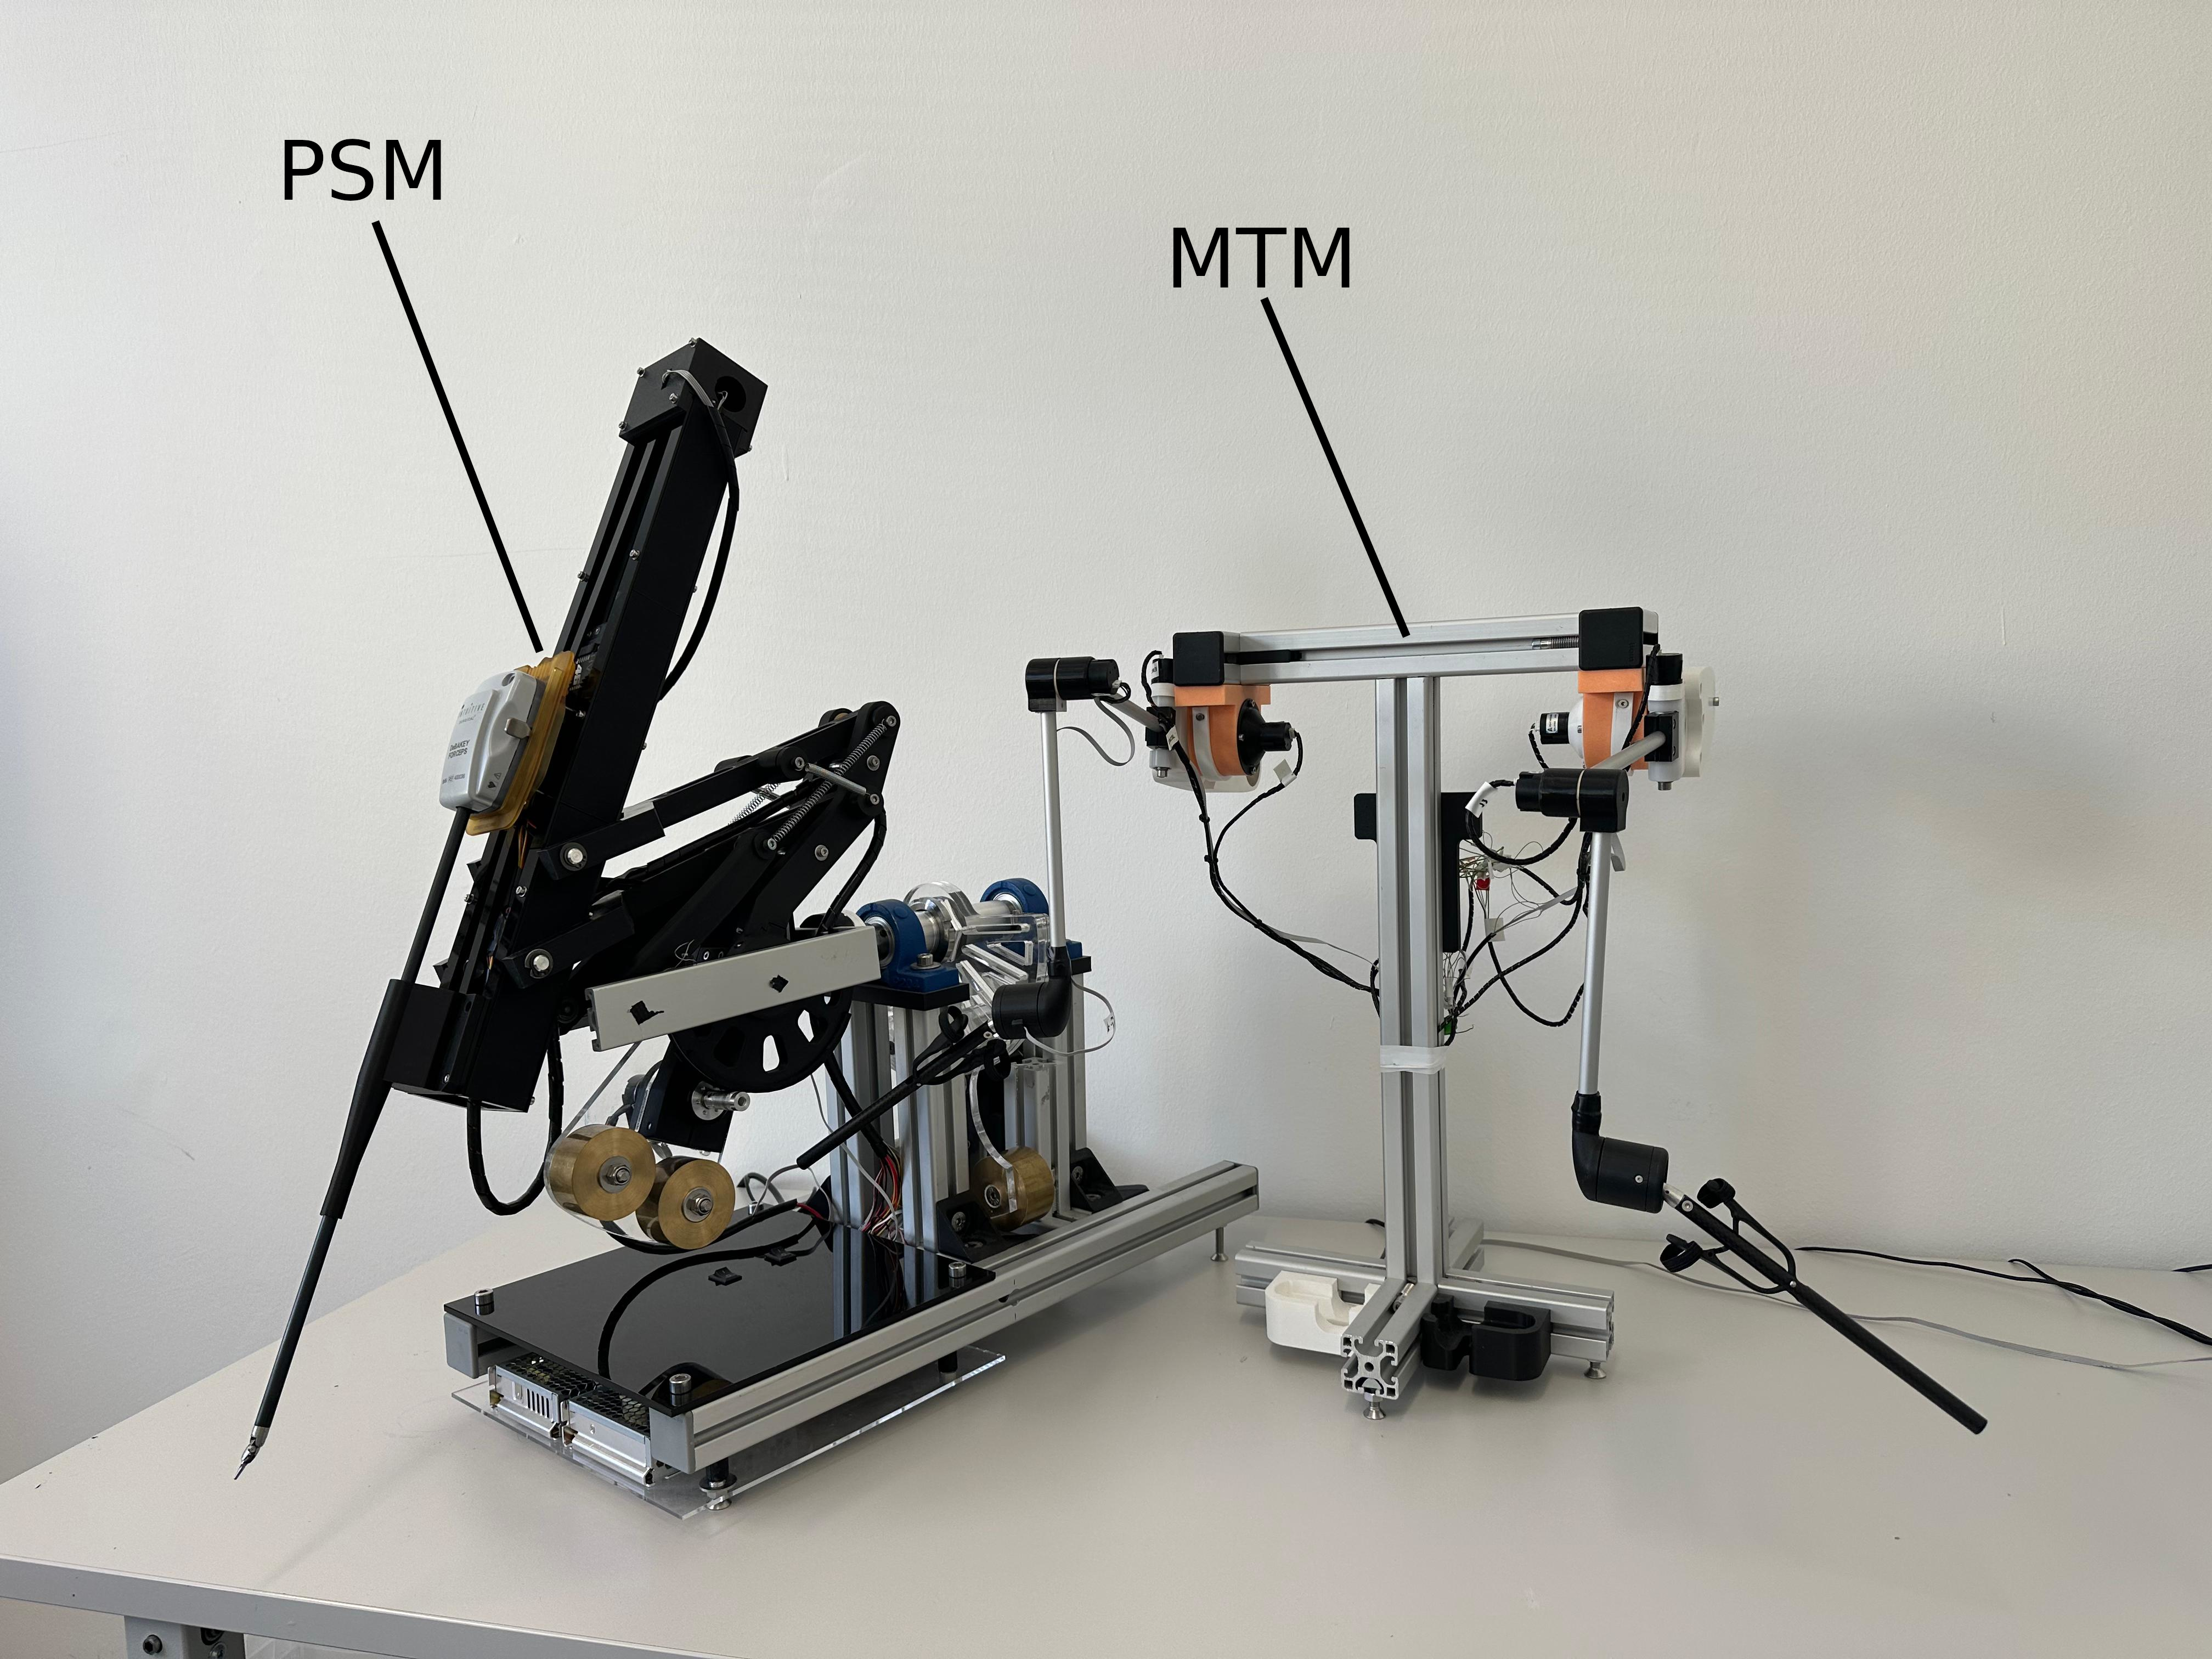
\includegraphics[width=0.75\linewidth]{figures/design/system_overview.png}
    \caption{Placeholder image of system}
    \label{fig:system_overview_placeholder}
\end{figure}


\section{MTM Mechanical Design}

The Master Tool Manipulator (MTM) can be separated into two subsystems:
\begin{itemize}
    \item Arm (J0-J2)
    \item Gimbal (G0-G3)
\end{itemize}

The arm subsystem refers to the overall architecture which is responsible for measuring the operator's position with respect to (w.r.t.) the global reference frame. Three revolute joints with internal optical encoders are coupled via rigid aluminum extrusions, allowing for accurate estimation of the overall system positioning in 3D space, as shown in Figure~\ref{fig:mtm_overview}.

\begin{figure}[h]
    \centering
    \includegraphics[width=0.75\linewidth]{figures/mtm_overview.png}
    \caption{Detailed depiction of the MTM's arm and wrist subsystems, with their individual components labeled.}
    \label{fig:mtm_overview}
\end{figure}

\subsection{Joints}
The arm of the manipulator consists of three revolute joints connecting the four links of the MTM arm. Table~\ref{tab:mtm_joints} summarizes these joints and provides a description of their function.

\begin{table}[h]
\centering
\caption{Summary and description of revolute (R) joints of the MTM's arm \cite{ref19,ref20}.}
\label{tab:mtm_joints}
\begin{tabular}{|c|c|l|p{8cm}|}
\hline
\textbf{MTM Joint} & \textbf{Joint Type} & \textbf{Joint Name} & \textbf{Description} \\
\hline
1 & R & Shoulder pitch & This joint moves the entire MTM and carries out pitch rotation similar to joint 3. \\
\hline
2 & R & Shoulder yaw & This joint is responsible for adduction and abduction movement of the operator. \\
\hline
3 & R & Elbow pitch & This joint is the second pitch joint of the MTM. Together with joint 1, it is responsible for up/down and forward/backward motion. \\
\hline
\end{tabular}
\end{table}

The design of these joints was driven by the requirement to minimize friction. Increased frictional forces in any of these joints would result in an increase in perceived force by the operator. As visible in Figure~\ref{fig:mtm_detailed}, roller bearings were utilized to minimize these frictional forces, and system mass was also reduced to lower both gravitational and inertial forces felt by the operator.

\begin{figure}[h]
    \centering
    \includegraphics[width=0.75\linewidth]{figures/mtm_detailed.png}
    \caption{Exploded view of the MTM components (excluding EWCU fixation) showing the updated training console design. Key improvements include: (1) circlip for axial safeguarding, (2) PTFE thrust washer to eliminate bearing clearance effects while maintaining low friction, and (3) reduced wear characteristics.}
    \label{fig:mtm_detailed}
\end{figure}


\section{MTM Electrical Architecture}

\subsection{System Overview}
The MTM (Master Tool Manipulator) electrical architecture was originally based around an Arduino Mega 2560 microcontroller that served as both the primary controller and system I/O interface. This configuration was later upgraded to a Teensy 4.1 microcontroller due to its superior performance and compatibility with ROS2 and micro-ROS frameworks.

The system incorporates multiple sensor subsystems to monitor and control the robotic arm's movements. Each side of the arm is equipped with sensors for:
\begin{itemize}
    \item Shoulder pitch (J0)
    \item Shoulder yaw (J1)
    \item Elbow pitch (J2)
    \item Wrist orientation (G0-G2)
    \item Grasper state (G3)
\end{itemize}

\subsection{Joint Subsystems (J0-J2)}
Joints J0-J2 are equipped with AEAT-6012-A06 12-bit absolute magnetic encoders (resolution: 4096 counts/revolution) directly coupled to each joint axis. These encoders provide a positional accuracy of $\pm 0.088^\circ$ ($360^\circ/4096$) per joint, enabling precise positional feedback for the control system.

\begin{itemize}
    \item \textbf{Shoulder Pitch (J0)}: Magnetic encoder provides precise feedback on shoulder pitch position
    \item \textbf{Shoulder Yaw (J1)}: Magnetic encoder measures shoulder yaw angle
    \item \textbf{Elbow Pitch (J2)}: Magnetic encoder monitors elbow pitch movement
\end{itemize}

The encoder signals are connected directly to the Teensy 4.1's digital I/O pins through a noise-resistant shielded cable assembly.

\subsection{Wrist Subsystem (G0-G3)}
The wrist subsystem underwent significant design evolution:
\begin{itemize}
    \item \textbf{Initial Design}: Utilized an MPU-6050 IMU (3-DOF) for wrist orientation sensing and a Hall effect sensor for grasper state detection
    \item \textbf{Issues Encountered}: Noticeable drift occurred in the IMU during prolonged operation
    \item \textbf{Final Implementation}: Replaced with analog potentiometers for wrist position detection (G0-G2) while retaining the Hall effect sensor for grasper state detection (G3)
\end{itemize}

The MPU-6050 IMU provided the following measurement capabilities:
\begin{itemize}
    \item 3-axis accelerometer ($\pm 2/4/8/16$ g configurable)
    \item 3-axis gyroscope ($\pm 250/500/1000/2000^\circ$/s configurable)
\end{itemize}

\subsection{Connectivity}
All wrist sensors (G0-G3) connect to the Teensy 4.1's analog I/O pins through a 7-strand flat flexible cable (FFC) with the following specifications:
\begin{itemize}
    \item Pitch: 0.5mm
    \item Current rating: 0.3A per conductor
    \item Voltage rating: 50V
    \item Temperature range: $-40^\circ$C to $+105^\circ$C
\end{itemize}

\subsection{Grip Subsystem}
The grip detection system utilizes a Hall effect sensor to measure the position between the index finger and thumb components. Key characteristics include:
\begin{itemize}
    \item Sensing range: $\pm 50$mm
    \item Resolution: 0.1mm
    \item Output: Analog voltage (0-3.3V)
\end{itemize}

\section{PSM Mechanical Design}

\subsection{Overview}
The Patient-Side Manipulator (PSM) mechanical architecture is a 7-degree-of-freedom (DOF) robotic system designed to replicate surgical instrument movements with high precision. The design is fundamentally inspired by the da Vinci Surgical System's remote center of motion (RCM) mechanism, which maintains a fixed pivot point at the surgical incision site - a critical feature for minimally invasive surgery. The PSM can be divided into five primary subsystems:

\begin{itemize}
    \item Superstructure and base
    \item Roll (yaw) axis
    \item Pitch axis
    \item Insertion axis
    \item Tool cart and end effector
\end{itemize}

\subsection{Superstructure}
The superstructure serves as the foundational framework, constructed from 80/20 aluminum extrusion for both rigidity and modularity. This design provides:
\begin{itemize}
    \item Structural stability for the entire system
    \item Mounting points for all electromechanical components
    \item Vibration damping through its triangulated geometry
    \item Accessibility for maintenance and upgrades
\end{itemize}

The aluminum extrusion profile (40mm × 40mm, series 8) was selected for its excellent strength-to-weight ratio and compatibility with standard motion components.

\subsection{Roll (Yaw) Axis}
The roll axis implements a revolute joint providing $\pm$90$^\circ$ of rotation about the vertical axis, corresponding to the da Vinci system's first DOF.

\begin{itemize}
    \item \textbf{Drive System}: Maxon EC-4pole 30 brushless DC motor (50W) coupled to a 20:1 Capstan drive
    \item \textbf{Transmission}: Zero-backlash Capstan drive (0.1 arc-minute repeatability)
    \item \textbf{Bearing System}: Two NSK LH-series linear bearing blocks supporting a 16mm ground aluminum shaft
    \item \textbf{Position Sensing}: Broadcom HEDS-5540 optical encoder (500 CPR)
    \item \textbf{Safety}: Omron D2F-L-A1 limit switches at $\pm$90$^\circ$ travel limits
\end{itemize}

The roll axis terminates in an aluminum fork structure that supports both the pitch and insertion axes, maintaining the kinematic chain.

\subsection{Pitch Axis}
The pitch axis replicates the da Vinci's characteristic parallelogram mechanism, which creates a virtual RCM approximately 50mm distal to the joint - matching typical trocar insertion depths.

\begin{itemize}
    \item \textbf{Mechanism}: Dual-parallelogram linkage with 3D-printed ABS components
    \item \textbf{Drive System}: Maxon EC-4pole 30 motor with identical 20:1 Capstan drive
    \item \textbf{Range of Motion}: $\pm$45$^\circ$ from neutral position
    \item \textbf{Advantages}:
        \begin{itemize}
            \item Maintains constant instrument orientation during arm motion
            \item Creates natural RCM without complex constrained mechanisms
            \item Reduces shear forces at the incision point
        \end{itemize}
\end{itemize}

The 3D-printed design (Prusa MK3S+, 0.15mm layer height) was chosen for rapid prototyping and weight reduction, with critical joints reinforced with stainless steel pins.

\subsection{Insertion Axis}
The prismatic insertion axis provides 200mm of linear travel, corresponding to the da Vinci's third DOF.

\begin{itemize}
    \item \textbf{Drive Mechanism}: HV7346MG servo (modified for continuous rotation) with rack-and-pinion transmission
    \item \textbf{Guide System}: IGUS drylin linear rails (model RJ4JP-01-08)
    \item \textbf{Position Sensing}: Integrated optical encoder with 0.1mm resolution
    \item \textbf{Safety}: Dual Omron limit switches at travel extremes
\end{itemize}

The rack-and-pinion system (module 0.5, 20$^\circ$ pressure angle) provides 96.5\% efficiency while maintaining the compact form factor required for surgical applications.

\subsection{Tool Cart and End Effector}
The tool cart integrates four degrees of freedom in a package matching Intuitive Surgical's instrument specifications:

\begin{itemize}
    \item \textbf{Actuation}: Four MG966R servos with spring-loaded coupling mechanisms
    \item \textbf{Functions}:
        \begin{itemize}
            \item Instrument roll ($\pm$90$^\circ$)
            \item Wrist pitch ($\pm$85$^\circ$)
            \item Wrist yaw ($\pm$85$^\circ$)
            \item Grasper actuation (0-100\%)
        \end{itemize}
    \item \textbf{Instrument Interface}: Compatible with Intuitive Surgical EndoWrist\textsuperscript{\textregistered} tools
    \item \textbf{Coupling Mechanism}: Fail-safe magnetic coupling with 5N retention force
\end{itemize}

\subsection{Remote Center of Motion Implementation}
The PSM's mechanical architecture replicates the da Vinci system's key innovation - the passive RCM mechanism. This is achieved through:

\begin{itemize}
    \item \textbf{Parallelogram Linkage}: Mathematically constrains motion to a fixed point
    \item \textbf{Kinematic Design}: Aligns axes to intersect at the RCM point
    \item \textbf{Clinical Benefits}:
        \begin{itemize}
            \item Minimizes tissue trauma at incision site
            \item Provides intuitive instrument control
            \item Reduces fulcrum effect during manipulation
        \end{itemize}
\end{itemize}


\section{PSM Electrical Architecture}

\subsection{System Overview}
The Patient-Side Manipulator (PSM) electrical architecture is designed to meet stringent surgical robotic requirements, including:
\begin{itemize}
    \item Sub-millimeter positional accuracy ($\pm$0.2mm at instrument tip)
    \item High dynamic response (bandwidth > 10Hz for all axes)
    \item Fail-safe operation with redundant position verification
    \item Low-latency control loops ($<$1ms cycle time)
\end{itemize}

The system implements a distributed control architecture centered around a Teensy 4.1 microcontroller (600MHz ARM Cortex-M7), chosen for its:
\begin{itemize}
    \item Real-time performance capabilities
    \item Extensive I/O options (28 PWM channels, 16 analog inputs)
    \item Native USB 2.0 support for ROS2 integration
    \item FPU support for advanced control algorithms
\end{itemize}

\subsection{Position Sensing System}
\subsubsection{Primary Joint Sensing}
\begin{itemize}
    \item \textbf{Roll/Yaw Axis}: Broadcom HEDS-5540 optical encoder (500 CPR) with quadrature decoding
    \item \textbf{Pitch Axis}: Broadcom HEDS-5540 optical encoder (500 CPR)
    \item \textbf{Insertion Axis}: AMS AS5047P magnetic encoder (14-bit resolution, 0.022$^\circ$ accuracy)
\end{itemize}

\subsubsection{Secondary Verification}
\begin{itemize}
    \item Omron D2F-L-A1 mechanical limit switches at all travel extremes
    \item Current sensing via INA219 shunt monitors (0.5\% accuracy)
    \item Thermal monitoring on all motor drivers
\end{itemize}

\subsection{Motor Drive System}
\subsubsection{Main Axes Actuation}
\begin{table}[h]
\centering
\caption{Main Axes Drive Specifications}
\begin{tabular}{|l|c|c|c|}
\hline
\textbf{Parameter} & \textbf{Roll} & \textbf{Pitch} & \textbf{Insertion} \\ \hline
Motor & Maxon EC-4pole 30 & Maxon EC-4pole 30 & HV7346MG \\
Voltage & 24V & 24V & 12V \\
Continuous Current & 2.5A & 2.5A & 3.2A \\
Peak Torque & 50mNm & 50mNm & 15kg-cm \\
Driver & MD13S Cytron & MD13S Cytron & MD13S Cytron \\
Control Mode & PID Velocity & PID Position & PID Position \\
Bandwidth & 500Hz & 500Hz & 300Hz \\ \hline
\end{tabular}
\end{table}

\subsubsection{Servo Control Implementation}
The wrist subsystem utilizes four MG966R servos modified for continuous rotation and external position control:
\begin{itemize}
    \item \textbf{Control Method}: PWM (1-2ms pulse width) with 12-bit resolution
    \item \textbf{Position Feedback}: Internal potentiometer (10k$\Omega$, 300$^\circ$ range)
    \item \textbf{External Verification}: AS5600 magnetic encoders on output shafts
    \item \textbf{Spring Coupling}: 0.5N/mm preloaded springs ensure zero backlash
\end{itemize}

\subsection{Safety and Calibration}
The system implements a comprehensive safety architecture:
\begin{itemize}
    \item Dual-channel limit switch verification (mechanical + optical)
    \item Watchdog timer (100ms timeout) on all motor drivers
    \item Current limiting at both driver and software levels
    \item Automatic homing sequence on startup:
    \begin{enumerate}
        \item Seek limit switch at reduced velocity (10\% max)
        \param{Back off 5mm from limit}
        \item Establish encoder zero position
    \end{enumerate}
\end{itemize}

\subsection{Control Architecture}
The Teensy 4.1 implements the following control scheme:
\begin{itemize}
    \item \textbf{Sampling Rate}: 1kHz for all critical loops
    \item \textbf{Algorithm}: Adaptive PID with velocity feedforward
    \item \textbf{Communication}:
    \begin{itemize}
        \item ROS2 interface (micro-ROS) @ 100Hz
        \item CAN bus for motor drivers (1Mbps)
        \item I$^2$C for sensors (400kHz fast mode)
    \end{itemize}
    \item \textbf{State Estimation}: Kalman filter combining encoder and IMU data
\end{itemize}

\subsection{Power Distribution}
\begin{itemize}
    \item \textbf{Main Bus}: 24V DC (Mean Well LRS-350-24)
    \item \textbf{Logic Power}: 5V/3A buck converter (TI TPS5430)
    \item \textbf{Protection}:
    \begin{itemize}
        \item Polyfuses on all outputs
        \item TVS diodes for surge protection
        \item Star grounding for noise reduction
    \end{itemize}
\end{itemize}

\section{System Software Architecture}
\label{sec:software_architecture}

As noted earlier in this paper, the initial software framework was implemented in an Arduino C-based environment. While the system has since been migrated to a ROS 2 architecture, the original implementation remains relevant for context and reference.

The software was divided into two primary components: the \textbf{Master Tool Manipulator (MTM)} software and the \textbf{Patient Side Manipulator (PSM)} software. These subsystems worked in tandem to enable real-time teleoperation, with the MTM capturing user inputs and the PSM replicating movements precisely.

\subsection{MTM Software}
The MTM software was responsible for:

\begin{enumerate}
    \item \textbf{Sensor Data Acquisition}:
    \begin{itemize}
        \item Reading six absolute magnetic encoders, two IMUs (Inertial Measurement Units), and two Hall effect sensors (eight sensor values per MTM arm)
        \item Distinguishing between left and right-arm data for independent kinematic processing
    \end{itemize}
    
    \item \textbf{Forward Kinematics}:
    \begin{itemize}
        \item Calculating the system's position and orientation from raw sensor data
        \item Smoothing noisy signals using low-pass filters (\texttt{LPFilter.ino}, \texttt{LPFilter\_Encoder.ino})
    \end{itemize}
    
    \item \textbf{Data Processing and Safety}:
    \begin{itemize}
        \item Detecting abrupt movements via spike detection logic (\texttt{spikeDetection.ino})
        \item Monitoring sensor overflow conditions (\texttt{OverFlowDetection.ino})
    \end{itemize}
    
    \item \textbf{Communication}:
    \begin{itemize}
        \item Relaying processed kinematic data to the PSM via serial communication
        \item Packaging data with start/end markers for robust parsing (\texttt{recvWithStartEndMarkers.ino})
    \end{itemize}
\end{enumerate}

\textbf{Key files included}:
\begin{itemize}
    \item \texttt{MT\_MTM.ino}: Central coordination, subsystem integration, and communication with the Arduino Mega
    \item \texttt{KinematicCalc\_L/R.ino}: Arm-specific forward kinematics for joint angle derivation
    \item \texttt{readIMU.ino} \& \texttt{readEncoder.ino}: IMU quaternion and encoder position data handling
\end{itemize}

\subsection{PSM Software}
The PSM software replicated MTM movements using:

\begin{enumerate}
    \item \textbf{Data Reception and Parsing}:
    \begin{itemize}
        \item Extracting target positions from serial messages (\texttt{parseData.ino})
    \end{itemize}
    
    \item \textbf{Closed-Loop Control}:
    \begin{itemize}
        \item Executing PID control for motor actuation (\texttt{PIDupdate.ino})
        \item Implementing ramp-up routines for smooth motion initiation (\texttt{RampUp\_Homing.ino})
    \end{itemize}
    
    \item \textbf{Safety and Calibration}:
    \begin{itemize}
        \item Collision detection via limit switches (\texttt{CheckCol.ino})
        \item Reference drives for incremental encoders (joints 1--3) to establish absolute positioning post-startup
        \item Tool manipulation routines (\texttt{Catch\_Tool.ino}) and PWM frequency tuning (\texttt{setPwmFrequency.ino})
    \end{itemize}
\end{enumerate}

\section{System Kinematics and Coordinate Frames}

\section{System PID Controller Design}



\chapter{Implementation on Current Hardware}

\section{Software Architecture}

This section will serve as an overview of the current system software architecture and will provide an in-depth analysis of how the current ROS2 Node structure works.

\subsection{ROS 2 System Architecture}

The current system's ROS 2 architecture is composed of four primary nodes, each responsible for specific functionalities:

\begin{itemize}
    \item \textbf{MTM Node (Micro-ROS):} This node is responsible for streaming sensor data from the Master Tool Manipulator (MTM) and performing forward kinematics calculations to determine the target pose.
    \item \textbf{System Model Node:} This node maintains a Simulation Description Format (SDF) model of the MTM. It facilitates real-time visualization of the system's configuration and enables the calculation of various joint frames.
    \item \textbf{Joint Publisher Node:} Acting as an intermediary, this node utilizes the SDF model to offer an alternative method for calculating the target position based on TF (Transform Frame) transformations.
    \item \textbf{PSM Node (Micro-ROS):} This node handles sensor data acquisition, implements control logic, and drives the Patient Side Manipulator (PSM) system.
\end{itemize}

\begin{figure}[h!]
    \centering
    \begin{tikzpicture}[node distance=1cm, auto] % Reduced node distance for a narrower figure
        % Nodes
        \node (mtm) [block] {MTM Node};
        \node (sdf) [block, right=of mtm] {SDF Model};
        \node (jointpub) [block, right=of sdf] {Joint Publisher Node};
        \node (psm) [block, right=of jointpub] {PSM Node};

        % Arrows
        \draw[arrow] (mtm) -- (sdf);
        \draw[arrow] (sdf) -- (jointpub);
        \draw[arrow] (jointpub) -- (psm);
    \end{tikzpicture}
    \caption{Initial ROS 2 System Architecture for Target Pose Calculation.}
    \label{fig:initial_architecture}
\end{figure}

Initially, the research aimed for the MTM Node to relay its joint angles to the SDF Model of the MTM. Subsequently, the Joint Publisher Node would calculate the desired end-effector position via a TF frame transformation from the base frame to the gimbal origin. This approach was intended to provide an alternative method for extracting the target position, bypassing the need for explicit forward kinematics in the MTM node. This architecture is illustrated in Figure \ref{fig:initial_architecture}. While this method proved effective in accurately calculating the target pose, real-time performance trials revealed significant limitations.

Specifically, although the target position extracted from the model demonstrated excellent real-time performance, a communication protocol breakdown was observed when the Joint Publisher Node interfaced with the Micro-ROS PSM Node. This breakdown was likely caused by memory limitations inherent to the Teensy 4.1 microcontroller, leading to high latency and noticeable data stuttering.

---

Consequently, a simplified architecture was explored to overcome these real-time performance issues. This revised approach involves performing forward kinematics calculations of the target position directly within the MTM Node and streaming this data topic directly to the PSM Node. This simplification of the technical stack significantly improved real-time performance and reduced system complexity. This optimized architecture is presented in Figure \ref{fig:optimized_architecture}.

\begin{figure}[h!]
    \centering
    \begin{tikzpicture}[node distance=2.5cm, auto]
        % Nodes
        \node (mtm) [block] {MTM Node};
        \node (psm) [block, right=of mtm] {PSM Node};

        % Arrows
        \draw[arrow] (mtm) -- (psm);
    \end{tikzpicture}
    \caption{Optimized ROS 2 System Architecture for Direct Target Pose Streaming.}
    \label{fig:optimized_architecture}
\end{figure}

\subsection{MTM Modeling and Visualization}

For the modeling of the MTM, the Simulation Description Format (SDF) was chosen due to its compatibility with ROS 2 and RViz. SDF also supports complex kinematic structures, including closed-chain kinematics, which is crucial for accurately modeling the more intricate four-bar style linkages found in the Patient Side Manipulator (PSM).

Generating the SDF file proved to be a fairly involved process. First, the CAD model of the MTM system was imported into SolidWorks. To reduce computational complexity, the model underwent significant simplification. Parts were condensed into their respective links, identified as follows:

\begin{itemize}
    \item Base
    \item J1 (Joint 1)
    \item J2 (Joint 2)
    \item J3 (Joint 3)
    \item G3 (Gimbal Link 3)
    \item G2 (Gimbal Link 2)
    \item G1 (Gimbal Link 1)
    \item G0 (Gimbal Link 0)
\end{itemize}

Each of these components was created as a singular solid part and then reassembled within SolidWorks into a complete assembly.

Following this, rotational axes and origins were assigned for each link. A SolidWorks plugin was then utilized to export the model into a Universal Robot Description Format (URDF) file. This URDF file was subsequently converted to SDF using a dedicated software tool, \textit{ros2\_sdf\_to\_urdf} (further citation needed). Upon the successful generation of the SDF model, a Python launch file was developed to facilitate quick and easy visualization of this model within RViz.

The final result of this effort can be seen below in Figure \ref{fig:mtm_sdf_model}.

\begin{figure}[h]
    \centering
    \includegraphics[width=0.75\linewidth]{figures/mtm_sdf_model.png}
    \caption{SDF model of MTM}
    \label{fig:mtm_sdf_model}
\end{figure}

\subsection{MTM Data Streaming and filtering}

The MTM node's primary purpose is to process incoming sensor data and broadcast it into the \texttt{ROS2} workspace in a usable format. The following topics are published into the \texttt{ROS2} workspace from the MTM:

---

The MTM node's primary purpose is to process incoming sensor data and broadcast it into the \texttt{ROS2} workspace in a usable format. The following topics are published into the \texttt{ROS2} workspace from the MTM:

---

\begin{table}[h!]
    \centering
    \caption{MTM \texttt{ROS2} Topics}
    \label{tab:mtm_ros2_topics}
    \begin{tabular}{|l|l|p{5cm}|} % Changed to p{5cm}
        \hline
        \textbf{Topic Name} & \textbf{Topic Type} & \textbf{Description} \\
        \hline
        \texttt{mtm\_joint\_states} & \texttt{sensor\_msgs/msg/JointState} & Current angular positions for all robotic arm joints. \\
        \hline
        \texttt{mtm\_raw\_values} & \texttt{std\_msgs/msg/Float32MultiArray} & Unfiltered raw sensor data for debugging. \\
        \hline
        \texttt{12target\_pose} & \texttt{sensor\_msgs/msg/JointState} & Calculated Cartesian (x, y, z) position of the end-effector in meters. \\
        \hline
    \end{tabular}
\end{table}

\subsection{MTM to PSM Communication Protocol}

As previously established in Section 4.1, there are two separate paths for data communication between the MTM and the PSM: the direct communication path and the path utilizing the SDF model as an intermediary.

A critical aspect of both communication paths is ensuring **Quality of Service (QoS)** protocol matching. QoS allows for the definition of how topics are communicated between nodes. Ensuring that communicating nodes utilize appropriate and compatible QoS protocols is essential for software reliability and robustness. For this research, the QoS reliability and queue depth were modified to ensure proper message delivery.

Initially, an issue arose with the communication protocol between the SDF model and the PSM node. Data streamed from the SDF model was published to the \texttt{/model\_pose} topic. When this data was plotted, it exhibited high quality with zero latency or lag. However, when the PSM topic \texttt{/psm\_joint\_telemetry} subscribed to \texttt{/model\_pose}, a significant loss of data occurred, resulting in lag and stuttering. This led to unacceptable system performance. After extensive diagnostics, the data performance was improved by drastically increasing the publishing rate from 100\,Hz to 1000\,Hz, increasing the queue depth from 10 to 20, and applying the following QoS profile:

\begin{itemize}
    \item \textbf{Reliability:} \texttt{RELIABLE}
    \item \textbf{History (Depth):} 20
    \item \textbf{Durability:} \texttt{VOLATILE}
    \item \textbf{Lifespan:} Infinite
    \item \textbf{Deadline:} Infinite
    \item \textbf{Liveliness:} \texttt{AUTOMATIC}
    \item \textbf{Liveliness lease duration:} Infinite
\end{itemize}

Increasing the publishing rate to such a drastic level required careful memory consideration to avoid overwhelming the limited memory of the PSM's Teensy 4.1. As a result, the \texttt{model\_pose} message type was changed from a \texttt{JointTelemetry} message type to a \texttt{JointState} message type to reduce memory strain.

\begin{figure}
    \centering
    \includegraphics[width=0.5\linewidth]{figures/bad_data.png}
    \caption{Enter Caption}
    \label{fig:bad_data_placeholder}
\end{figure}
\subsection{PSM Software}


\section{System Identification}

For this research, proper controller design was paramount. However, a high-performance controller could not be designed without a fundamental understanding of the system's dynamics. To achieve this, a robust system identification scheme was developed.

The two primary joints of interest were the roll and pitch joints. These joints exhibited complex system dynamics and a high degree of nonlinearity. An exact system identification approach was tailored to each joint's unique dynamics.

\subsection{Roll Joint Open loop Step Response}

The roll joint can be mechanically described as a pendulum. Perturbations applied to the system move the joint away from its $0^\circ$ position, but when the perturbation ceases, gravitational forces return the joint to its $0^\circ$ position. The system was also determined to have a fairly consistent and predictable transfer function. Specifically, when the brushless motor was driven at a specific voltage, the resulting positional change of the system was consistent across trials. As a result of these factors, a step response characterization was deemed an excellent method for system identification.

A step response characterization is a common system identification method in control engineering. In this technique, the system's input is abruptly changed from one value to another, and the resulting system response is measured and used to characterize the system's dynamics.

For the roll axis, a very lightly tuned PID controller was initially employed to drive the system to the intended point of characterization. A predetermined delay allowed the system to settle into a stable state. Upon completion of this delay, the current motor voltage value was stored, then scaled by a factor of 1.1 before being sent to the motor. Both the motor voltage input over time and the positional output of the roll joint over time were recorded. This system response data was saved as a CSV file and subsequently loaded using a custom MATLAB script. This script parsed the data and then fitted a second-order transfer function to the system response using MATLAB's \texttt{tfest} command. Finally, state-space matrices could then be extracted from this transfer function using MATLAB's \texttt{ss} command.



\subsection{Closed loop excitation through PRBS}

Initial characterization of the pitch subsystem used a similar approach to the roll subsystem. A step response was applied, and the resulting response was used to characterize the system. However, several issues were found with the step response characterization of the pitch subsystem.

Due to the mechanical nature of the joint, the pitch subsystem's response was highly nonlinear. A slight change in voltage applied to the motor resulted in large changes in the pitch system's position, and this behavior was not consistent between trials. The same change in motor voltage would not result in the same system response. Additionally, when a small increase in voltage was applied to a stable system position, the pitch subsystem would drive to the end of its range of motion and contact the hard stop. This overshooting was a result of the pitch subsystem's extremely sensitive system response as its angle increased. This sensitivity was a direct consequence of the mechanical design of the pitch subsystem, where the force applied by the gravity compensation system drastically reduced as the angle of the pitch subsystem increased.

As a result of these complexities, a different approach had to be implemented. Due to the difficulties in maintaining the pitch subsystem within its intended range of motion, it was deduced that system identification needed to be conducted under closed-loop system control.

For this system identification technique, a light PD controller was applied to the system. The system was then commanded to its intended characterization point. Upon a predetermined settling time, the control input was then excited with a Pseudo-Random Binary Sequence (PRBS).

PRBS is a control signal excitation technique in which the control input is randomly fluctuated by a set amplitude at pseudo-random, predetermined intervals. By exciting the control input, the resulting behavior and system dynamics could be observed while the aforementioned PD controller attempted to bring the system back to its setpoint. Key considerations in closed-loop PRBS excitation are ensuring that the amplitude of the excitation is sufficient to bring the system off its setpoint and overcome noise, while also ensuring that the amplitude of the excitation does not overpower the controller and drive the system off its setpoint. Additionally, the intervals between the fluctuations of the excitation need to be chosen such that the system's dynamics are excited across a variety of frequencies.

To ensure that the system undergoes excitation at all critical frequencies multiple times, the PRBS characterization was run for an extended period. Trials typically lasted 30-660 seconds. During these trials, the pitch subsystem's input voltage and resulting position were continuously recorded. This output data was saved as a CSV file, and an additional MATLAB script was used to perform a mathematical characterization of the system.

Similarly to the roll subsystem, the recorded output of the pitch subsystem was loaded into a MATLAB script, and a variety of system identification techniques were applied to the data.

From these results, it was determined that a 4th-order transfer function estimation was the best method for characterizing the system.

After a 4th-order transfer function was fitted to the system using the MATLAB \texttt{tfest} command, the state-space matrices were extracted using the \texttt{ss} command. The estimated model's accuracy was then determined by comparing the actual system behavior based on the input to the predicted system behavior based on the system input using the MATLAB \texttt{compare} command.

From this comparison, it was determined that the model accuracy was quite low when compared to the real system response based on the input. However, when a controller was designed around this model estimation, the actual system performance was quite good. So, while this poor system estimation may point towards some underlying issues in the system identification technique, it ultimately resulted in a high-performing controller, which was the ultimate goal of this research.


\subsection{Multi-point System Identification}

Due to the kinematics of the system, the force required of the motors at various joint positions will vary. As the roll angle diverges farther from 0 in both the negative and positive direction, there is an increase in gravitational forces seen by the actuators, and as a result, the voltage applied to the motor would need to be increased accordingly. This trend is theoretically illustrated in Figure~\ref{fig:roll_voltage_trend}.

\begin{figure}[htbp]
    \centering
    \includegraphics[width=0.8\textwidth]{figures/Roll_Subsystem_Theoretical_Trend.png}
    \caption{Theoretical trend of absolute motor voltage required for the roll subsystem as a function of roll angle.}
    \label{fig:roll_voltage_trend}
\end{figure}

For the pitch subsystem, the force required by the actuator actually decreases as the joint moves through its range of motion from -30 degrees to 30 degrees. The theoretical voltage required for the pitch subsystem across its range of motion is shown in Figure~\ref{fig:pitch_voltage_trend}.

\begin{figure}[htbp]
    \centering
\includegraphics[width=0.8\textwidth]{figures/Pitch_Subsystem_Theoretical_Trend.png}
    \caption{Theoretical trend of required motor voltage for the pitch subsystem as a function of pitch angle.}
    \label{fig:pitch_voltage_trend}
\end{figure}

Additionally, complexities are added to the system dynamics when one realizes that the force required by the roll subsystem is also coupled to the pitch subsystem's position. As the pitch subsystem's angle is increased, the force required by the roll subsequently changes due to the system's center of mass changing position.

Similarly, the force required by the pitch subsystem varies with the position of the roll subsystem. As the roll subsystem diverges from the 0 point, the force required by the pitch subsystem lessens as it stays farther from its default position (normal to the gravitational force vector).

The combination of these factors necessitated the need for a more complex controller strategy in which the controller gains varied in accordance with the system position. The idea of this improved controller was that each joint's gains would vary with the current position of each subsystem.

This adaptive controller algorithm would require the characterization of the system at multiple points of the system's position. It was decided that 9 characterization points would be used for each joint of the subsystem. The pitch would be varied from $-15^\circ$, $0^\circ$, $15^\circ$ and the roll subsystem would vary from $-20^\circ$, $0^\circ$, $20^\circ$. This resulted in the following grid of 9 characterization points:

\begin{table}[htbp]
    \centering
    \caption{Grid of 9 Characterization Points for System Identification}
    \label{tab:characterization_points}
    \begin{tabular}{c|ccc} % c for the first column, then 3 c's for the data columns
        \multicolumn{1}{c}{} & \multicolumn{3}{c}{\textbf{Roll Angle ($^\circ$)}} \\ % Empty cell, then multicolumn for Roll Angle
        \cmidrule(lr){2-4} % Line under Roll Angle
        \textbf{Pitch Angle ($^\circ$)} & \textbf{-20} & \textbf{0} & \textbf{20} \\ % Pitch Angle label, then Roll values
        \midrule % Line separating headers from data
        \textbf{-15} & $(-15, -20)$ & $(-15, 0)$ & $(-15, 20)$ \\
        \textbf{0}   & $(0, -20)$   & $(0, 0)$   & $(0, 20)$   \\
        \textbf{15}  & $(15, -20)$  & $(15, 0)$  & $(15, 20)$  \\
        \bottomrule
    \end{tabular}
\end{table}

Once the necessary characterization points were established, the system needed to be identified at each of these points for each joint, resulting in the necessary system identification procedures. The actual system identification process was fairly straightforward. The previously established strategy for each joint was used; the only difference was that the positional setpoint for each characterization point varied to ensure the joint not being characterized remained at the necessary setpoint. The controller designed around the $(0,0)$ characterization point was used. While it was found that the dynamic performance of the controller designed around the $(0,0)$ setpoint degraded as the system diverged farther from the original linearization point, this controller performed well enough in the case of a static setpoint that it could be used to hold the extreme angles required by the multi-point system identification.

Once the necessary characterization points were established, the system needed to be identified at each of these points for each joint, resulting in the necessary system identification procedures. The actual system identification process was fairly straightforward. The previously established strategy for each joint was used; the only difference was that the positional setpoint for each characterization point varied to ensure the joint not being characterized remained at the necessary setpoint. The controller designed around the $(0,0)$ characterization point was used. While it was found that the dynamic performance of the controller designed around the $(0,0)$ setpoint degraded as the system diverged farther from the original linearization point, this controller performed well enough in the case of a static setpoint that it could be used to hold the extreme angles required by the multi-point system identification.

Upon the completion of each system identification trial, the resulting system response was saved in a CSV file under the following format: \texttt{IDENTIFIEDJOINT\_ROLLANGLE\_PITCHANGLE.csv}. A MATLAB script was then used to parse each of these files, identify the system at that point, and store and plot the system identification results.

\section{Controller Theory and Design}
The controller design was paramount to this research; a high emphasis was placed on system performance, and proper controller design would directly drive this. As a result, a large amount of effort was put into both the design and tuning of the controller.

\subsection{Original PID Controller}

The system originally utilized a very basic PID controller. Tuning was conducted with the Ziegler-Nichols method, and the following gains were found for each subsystem:

\begin{table}[htbp]
    \centering
    \caption{Ziegler-Nichols PID Gains for Roll and Pitch Subsystems}
    \label{tab:pid_gains}
    \begin{tabular}{l c c c}
        \toprule
        \textbf{Subsystem} & \textbf{$k_p$} & \textbf{$k_i$} & \textbf{$k_d$} \\
        \midrule
        Roll               & 35             & 50             & 5              \\
        Pitch              & 60             & 110            & 5              \\
        \bottomrule
    \end{tabular}
\end{table}

However, with these values, when full PID control was used, the system would rapidly vibrate, leading to uncontrolled system behavior and unacceptable noise and vibration. Because of this, the original system was only ever used with PD control, and its performance suffered greatly. Following sinusoidal trajectories, it would frequently undershoot or overshoot the setpoint and responded poorly to perturbations. As a result, an improved controller method needed to be developed.


\subsection{Model Predictive Control (MPC)}

Initially, several types of controllers were considered for this system. Model Predictive Control (MPC) was initially considered, as the system was already partially modeled in the form of an SDF model. MPC uses a dynamic model of the system to predict system behavior and determine a cost-optimal control input based on the model dynamics. While this control technique would result in extremely robust and optimal control, two factors prevented its utilization. First, the system model was a purely geometrical model, only accounting for the mass and inertia properties. Internal dynamics, such as frictional forces, were not considered, and the complexities of modeling such behavior were daunting. Secondly, MPC requires high computational power to simultaneously run and predict the model's behavior. This system utilized low-cost hardware with limited computational resources and, as a result, lacked the computational power to perform MPC.

\subsection{Gain Scheduling and Adaptive Control}

It was clear that due to varying system dynamics across the system's range of motion, adaptive control or gain scheduling would be a very valuable asset in improving system performance. Adaptive control involves online estimation of unknown or time-varying system parameters, or direct adjustment of controller parameters based on real-time performance feedback. In contrast, gain scheduling is a pre-programmed approach where controller parameters are adjusted based on a known, measurable "scheduling variable."

With relatively little additional computational power and complexity, the control gains could be calculated and interpolated based on the system's position, making gain scheduling an excellent candidate for improving system performance.



\subsection{LQR and LQI Control}

Linear Quadratic Regulator (LQR) control and Linear Quadratic Integral (LQI) control are cost-optimal control algorithms that minimize a quadratic cost function. LQI control extends the efforts of LQR control by incorporating integral action, which reduces steady-state error and improves system performance.

Both of these control methods are well-suited to this research as they achieve a good balance of high system performance with minimal control efforts. LQR control was chosen for the roll joint, as it was found that its performance was more than adequate for the system. However, during testing of the pitch subsystem, it was found that the system was consistently undershooting the desired positional setpoint. It was found that an LQI controller would minimize this steady-state error and drastically improve performance.

The objective of LQR control is to find a control input $\mathbf{u}(t)$ that minimizes the following quadratic cost function:
$$ J_{LQR} = \int_{0}^{\infty} (\mathbf{x}^T(t) Q \mathbf{x}(t) + \mathbf{u}^T(t) R \mathbf{u}(t)) \, dt $$
where:
\begin{itemize}
    \item $\mathbf{x}(t)$ is the state vector.
    \item $\mathbf{u}(t)$ is the control input vector.
    \item $Q$ is a positive semi-definite weighting matrix for the states, penalizing deviations from the desired state (often the origin).
    \item $R$ is a positive definite weighting matrix for the control inputs, penalizing control effort.
\end{itemize}

For LQI control, the system is augmented with an integral of the error, and the cost function is similarly minimized. If $\mathbf{e}_I(t)$ represents the integral of the output error, the augmented state $\mathbf{x}_{aug}(t)$ includes the original states and the integral error. The cost function for LQI is then:
$$ J_{LQI} = \int_{0}^{\infty} (\mathbf{x}_{aug}^T(t) \tilde{Q} \mathbf{x}_{aug}(t) + \mathbf{u}^T(t) R \mathbf{u}(t)) \, dt $$
where $\tilde{Q}$ is the augmented weighting matrix for the states, including a penalty on the integral error to drive it to zero.


\subsection{Feedforward Control}

Feedforward control is a control method which attempts to anticipate changes or disturbances to the system's input. It was theorized that a feedforward control strategy could further reduce any remaining steady-state error in the pitch subsystem.

In order for feedforward control to be implemented, a model of the system must be constructed in the form of a specific matrix known as the $B^\dagger$ matrix. The $B^\dagger$ matrix is formulated through the Moore-Penrose pseudoinverse. It is formulated as follows:

Let $B$ be an $m \times n$ real or complex matrix. Its Singular Value Decomposition (SVD) is given by:
$$B = U \Sigma V^T$$
where:
\begin{itemize}
    \item $U$ is an $m \times m$ unitary (or orthogonal for real matrices) matrix whose columns are the left singular vectors of $B$.
    \item $\Sigma$ is an $m \times n$ rectangular diagonal matrix with non-negative real numbers on the diagonal, called the singular values of $B$, typically arranged in decreasing order.
    \item $V^T$ is an $n \times n$ unitary (or orthogonal for real matrices) matrix whose rows are the right singular vectors of $B$. ($V$ is the matrix of right singular vectors).
\end{itemize}

The \textbf{Moore-Penrose pseudoinverse} of $B$, denoted $B^\dagger$, is then defined as:
$$B^\dagger = V \Sigma^\dagger U^T$$
where $\Sigma^\dagger$ is an $n \times m$ matrix formed by taking the reciprocal of each non-zero singular value on the diagonal of $\Sigma$, and then transposing the matrix.

The pseudoinverse $B^\dagger$ is unique and provides a "least squares" solution to linear equations. For a system $Bx = y$, if an exact solution doesn't exist, $x = B^\dagger y$ provides the solution that minimizes $||Bx - y||_2$.

For the purpose of this research, this matrix could be calculated via the MATLAB command \texttt{pinv}. This command, when applied to the identified $B$ matrix from the system identification procedure, would result in the $B^\dagger$ matrix.


This procedure was conducted for each of the characterization points previously discussed. Upon calculation of the $B^\dagger$ matrix, this matrix is used to calculate $u_{ff}$ by multiplying the $B^\dagger$ matrix (pseudoinverse of the input matrix) with the sum of the system's $A$ matrix multiplied by the reference state and the time derivative of the reference state. This $u_{ff}$ is then scaled by a factor $\lambda$, which can be tuned from $0$ to $1.0$ to adjust the feedforward element of the controller.

The ultimate result of this control effort is to proactively cancel anticipated system dynamics and generate better system performance.

\subsection{Comprehensive Control Strategy}


The final controller for the system was a resulting combination of several of the control strategies previously discussed. Ultimately, for the roll joint, it was found that gain scheduling with an LQR controller provided adequate system performance. However, for the pitch subsystem, this method needed to be improved upon due to consistent steady-state error in the form of target undershooting. To remedy this, an LQI controller with feedforward implementation and gain scheduling was employed. These strategies led to drastic improvements in system performance.

\chapter{System evaluation}
\label{chapter:results}

\section{Overview of Experiments}
\label{section:experiment_overview}

\section{Trajectory Tracking Performance}
\label{section:trajectory_performance}

\section{Effect of Adaptive Control}
\label{section:adaptive_pso_results}

\section{Summary of Results}
\label{section:results_summary}
\chapter{Conclusion and Future Work}
\label{chapter:conclusion}

The research aims of this project were successfully achieved. The system software architecture was updated from an Arduino C-based implementation to a more modern ROS 2 software framework. Additionally, the overall system performance was drastically improved through more robust system identification and control methods.

\section{Key Findings}
\label{section:key_findings}

Updating the software framework provided few quantitative performance improvements; however, qualitatively, the system framework is now more scalable. The SDF model allows for future work in collision detection, and the node-based architecture of the ROS 2 system created a robust platform for future development.

The improved system identification and control methods provided clear performance gains. Both the maximum and average positional error seen by the system were drastically reduced in all trials, and the system achieved smooth and stable performance during trajectory tracking.


\section{Limitations}
\label{section:limitations}

Throughout this research, significant hardware limitations became apparent. The original system was designed for ease of manufacturing and assembly, which led to many components being 3D printed. While this method was a simple and low-cost way to create the complex geometries required, the low stiffness of the plastic parts resulted in poor system performance.

During movement, the end-effector tip could be seen oscillating, a behavior that would be unacceptable in clinical procedures. Furthermore, prolonged use revealed that the components exhibited plastic creep. Many linkages warped beyond their specified tolerances, causing binding within the system and, in some instances, overcoming press-fits and disassembling during operation. Finally, the capstan cable tension proved inconsistent, frequently loosening and rendering previous system identifications obsolete. 

Additionally the ROS 2 implementation is limited to core middleware functionalities, and some advanced features such as security enhancements are not fully explored. Finally due to resource constraints, long-term reliability and robustness tests were not conducted. These limitations highlight potential areas for future research to extend the applicability and performance of the system.


\section{Recommendations for Future Work}
\label{section:future_work}

Before further research is conducted, it is recommended that the system's hardware be improved. The superstructure of the joints should be redesigned for increased stiffness, and more robust assembly methods must be employed. Additionally, a more consistent tensioning method for the capstan drives should be implemented, or the reduction technique must be changed altogether.

\section{Final Remarks}

Despite its hardware shortcomings, the objectives of this research were achieved. The system's software architecture was updated to a modern ROS 2 standard, and its performance was greatly improved through more robust identification and control techniques. While the system still requires improvements before it can replicate clinical procedures, the research conducted in this paper lays the groundwork for future development.

%\selectlanguage{english} % Re-select English if previous chapters were in German

% --- Listings (Code/Pseudo-code) ---
% Literaturverzeichnis IEEE-gerecht
\bibliographystyle{IEEEtran}	
\bibliography{bibliography}
\ifthenelse{\boolean{english}}{\addcontentsline{toc}{chapter}{Bibliography}}{\addcontentsline{toc}{chapter}{Literaturverzeichnis}} % f"ugt den Eintrag "Abbildungsverzeichnis" im Inhaltsverzeichnis hinzu

\pagenumbering{Roman}
\setcounter{page}{\value{romancount}}

\newpage

% Abbildungsverzeichnis
\listoffigures
\ifthenelse{\boolean{english}}{\addcontentsline{toc}{chapter}{List of Figures}}{\addcontentsline{toc}{chapter}{Abbildungsverzeichnis}} % f"ugt den Eintrag "Abbildungsverzeichnis" im Inhaltsverzeichnis hinzu
\newpage

% Tabellenverzeichnis
\listoftables 
\ifthenelse{\boolean{english}}{\addcontentsline{toc}{chapter}{List of Tables}}{\addcontentsline{toc}{chapter}{Tabellenverzeichnis}} % f"ugt den Eintrag "Tabellenverzeichnis" im Inhaltsverzeichnis hinzu
\newpage



 % Includes code listings or similar content

% --- Appendices ---
\appendix % Starts the appendix section
    \input{appendix/Matlab.tex} % Includes MATLAB-related appendix content
    \input{appendix/Jupyter} % Includes Jupyter-related appendix content
    \chapter{Source Code Repositories}
\label{chap:source_code}

This chapter contains references to the public GitHub repositories containing the source code and models developed for this thesis.

\section{PSM Firmware}
\label{sec:psm_src}
Contains the source code for the Power Supply Module (PSM).
\vspace{0.5cm}
\textbf{Repository URL:} \url{https://github.com/liamjosephnolan/psm_src}

\section{MTM Firmware}
\label{sec:mtm_src}
Contains the source code for the Master Thesis Motor (MTM) controller.
\vspace{0.5cm}
\textbf{Repository URL:} \url{https://github.com/liamjosephnolan/mtm_src}

\section{MATLAB Scripts}
\label{sec:matlab_scripts}
Contains the MATLAB scripts used for system identification, controller design, and generating plots for this thesis.
\vspace{0.5cm}
\textbf{Repository URL:} \url{https://github.com/liamjosephnolan/thesis_matlab}

\section{MTM SDF Model}
\label{sec:mtm_sdf}
Contains the Simulation Description Format (SDF) model of the MTM for use in the Gazebo simulator.
\vspace{0.5cm}
\textbf{Repository URL:} \url{https://github.com/liamjosephnolan/mtm_sdf}

\section{MTM Joint Publisher}
\label{sec:mtm_joint_publisher}
Contains the source code for the ROS 2 node that acts as a bridge between the MTM Micro-ROS node and the Gazebo SDF model.
\vspace{0.5cm}
\textbf{Repository URL:} \url{https://github.com/liamjosephnolan/mtm_joint_publisher}
""

\end{document}